\bigskip

\noindent \textbf{Definition 1 (\textit{Abstract service})}. A \textit{abstract service} describes the small piece of function that can be performed by a cloud service. For instance, retrieve patients, DNA information and personal information. The \textit{abstract service} is defined as $A \ (\overline{I}; \ \overline{O})$ where: 
\begin{itemize}
\item $A$ is a name which identifies the \textit{abstract service}.
\item $\overline{I}$ and $\overline{O}$ are a set of comma-separated input and output parameters, respectively.
\end{itemize}
The table~\ref{table:abstractservices} exemplifies \textit{abstract services} concerning our medical scenario described in the section~\ref{sec:scenario}.
%
%
\begin{table}[]
\centering
\begin{tabular}{|l|p{8cm}|l|}
\hline
\multicolumn{1}{|c|}{\textbf{\textit{Abstract service} name}} & \multicolumn{1}{c|}{\textbf{Description}} \\ \hline
$A1 \ (x; \ y)$ & Given a disease name $x$, $A1$ returns a list of infected patients' id $y$. \\ \hline
$A2 \ (w; \ z)$ & Given a patient id $w$, $A2$ returns her DNA information $z$. \\ \hline
$A3 \ (w; \ a)$ & Given a patient id $w$, $A3$ returns her personal information $a$.\\ \hline
$A4 \ (x; \ r)$ & Given a disease name $x$, $A4$ returns the most affected region $r$. \\ \hline
\end{tabular}
\caption{List of \textit{abstract services}.}
\label{table:abstractservices}
\end{table}
\bigskip

\noindent \textbf{Definition 2 (\textit{Concrete service})}. A \textit{concrete service} is defined as a set of \textit{abstract services}, and by its \textit{quality measures} extracted from its SLA according to the grammar:
%
\begin{center}
\begin{math}
S (\overline{I}_{h}; \overline{O}_{h}) := A_{1}(\overline{I}_{1l}; \overline{O}_{1l}), A_{2}(\overline{I}_{2l}; \overline{O}_{2l}), ..,  A_{f}(\overline{I}_{fl}; \overline{O}_{fl})[M_{1},M_{2}, ..,M_{g}]
\end{math}
\end{center}
%
The left-hand of the definition is called the \textit{head}; and the right-hand is the \textit{body}. 
A \textit{concrete service} $S$ includes a set of input $\overline{I}$ and output $\overline{O}$ variables, respectively.
Variables in the \textit{head} are identified by $\overline{I}_{h}$ and $\overline{O}_{h}$, and called \textit{head} variables. 
They appear in the \textit{head} and in the \textit{body} definition. 
Variables appearing only in the \textit{body} are identified by $\overline{I}_{l}$ and $\overline{O}_{l}$, and are called \textit{local} variables.

\textit{Concrete services} are defined in terms of \textit{abstract services} ($A_{1}, A_{2}, .., A_{n}$), and they include a set of service's quality aspects (quality measures) ($M_{1},M_{2}, .., M_{g}$). 
These measures are extracted from the respective SLA exported by the service.
%
%
$M_{i}$ is in the form $x \otimes c$, where $x$ is a special class of identifiers associated to the services; $c$ is a constant; and $\otimes \in\lbrace \geq, \leq, =, \neq, <, >\rbrace$. For example, consider the following \textit{concrete service} $S1$ which retrieves infected patients given a disease: 
\begin{center}
\small
\begin{math}
S1(d; p) := A1(d; p)[availability > 99\%, \ price \ per \ call = 0.1\$]
\end{math}
\end{center}
%
$S1$ is written using the \textit{abstract service} $A1$ defined before.
$d$ and $p$ are \textit{head} variables. 
$Availability$ and $price per call$ are quality measures extracted from $S1$ SLA.
%
%The table~\ref{table:concreteservices} shows examples of \textit{concrete services} and their functionality considering the \textit{abstract services} described before.

%\begin{table}[]
%\centering
%\begin{tabular}{|p{6cm}|p{6cm}|}
%\hline
%\multicolumn{1}{|c|}{\textbf{\textit{Concrete service} name}} & \multicolumn{1}{c|}{\textbf{Description}} \\ \hline
%$S1(d?; p!) := A1(d; p)[availability > 99\%, \ price \ per \ call = 0.1\$]$  & Given a disease name $x$, $A1$ returns a list of infected patients' id $y$. \\ \hline
%$S2(d; p) := A1(d; p)[availability > 97\%, \ price \ per \ call = 0.2\$]$  & Given a patient id $w$, $A2$ returns her DNA information $z$. \\ \hline
%$S3(p?; dna!) := GetDNA(d?; dna!)[availability > 98\%, \ price \ per \ call = 0.1\$]$ & Given a patient id $w$, $A3$ returns her personal information $a$.\\ \hline
%$S4(p?; info!) := GetInfo(d?; dna!)[availability > 98\%, \ price \ per \ call = 0.1\$]$ & Given a disease name $x$, $A4$ returns the most affected region $r$. \\ \hline
%$S5(d; dna) := A1(d; p), \ GetDNA(p?; dna!)[availability > 98\%, \ price \ per \ call = 0.1\$]$ & Given a disease name $x$, $A4$ returns the most affected region $r$. \\ \hline
%\end{tabular}
%\caption{List of \textit{concrete services}.}
%\label{table:concreteservices}
%\end{table}

% ----------------------------------- DEFINITION 3 QUERY --------------------------------- %
\bigskip

\noindent \textbf{Definition 3 (\textit{Query})}.
A user \textit{query} $Q$ is defined as a set of \textit{abstract services}, a set of \textit{constraints}, and a set of \textit{user integration preferences} in accordance with the grammar:
%
\begin{center}
\small
\begin{math}
Q (\overline{I}_{h}; \overline{O}_{h}) := A_{1}(\overline{I}_{1l};
\overline{O}_{1l}), A_{2}(\overline{I}_{2l}; \overline{O}_{2l}), ..,  A_{n}(\overline{I}_{nl}; \overline{O}_{nl}),C_{1},C_{2}, .., C_{m}[P_{1},P_{2}, .., P_{k}]
\end{math}
\end{center}
%
The \textit{query} definition is similar to a \textit{concrete service} concerning the variables and \textit{abstract services}. In addition, queries have constraints over the input or output variables ($C_{1}, C_{2}, .., C_{m}$). These constraints are used while querying the databases. The user \textit{integration preferences} over the services or over service compositions are specified in $P_{1}, P_{2}, .., P_{k}$. $C_{i}$ and $P_{j}$ are in the form $x \otimes c$, where $x$ is a identifier; $c$ is a constant; and $\otimes \in\lbrace \geq, \leq, =, \neq, <, >\rbrace$.
%

User preferences can be of two types, single and composed. Single preferences
are associated directly to each service involved in the composition. Composed
preferences are linked to the entire composition. They are defined in terms of
single preferences. For instance, the total response time is a composed
preference obtained by adding the response time of each service involved in the composition.

Let us suppose a query specification based on the medical scenario (section \ref{sec:scenario}) in which doctor \textit{Marcel} wants to query the personal and DNA information from patients that were infected by \textit{flu}, using services with availability higher than 98\%, price per call less than 0.2\$ and integration total cost less than 5\$.
To achieve his needs, \textit{Marcel} should compose the \textit{abstract services} $A1$, $A2$ and $A3$ as follows. 
%The figure~\ref{fig:queryandservices} illustrates doctor \textit{Marcel's} query and six \textit{concrete services} specified in terms of \textit{abstract services} defined before (Table~\ref{table:abstractservices}).

\begin{center}
\small
$Q(dis; dna, info) := A1(dis; p), A2(p; dna), A3(p; info) \ d = ``flu'' $
\\
$[availability > 98\%, \ price \ per \ call < 0.2\$, \ total \ cost < 5\$]$
\end{center}

The \textit{Marcel's }\textit{query} plan begins by retrieving infected patients ($A1$). This operation returns patients' ids $p$. The \textit{abstract services} $A2$ and $A3$ use patient ids to return their DNA and personal information ($dna$ and $info$).
%\textit{A user wants to retrieve patients DNA and personal information from patients infected by the disease ``flu'', using services with availability higher than 98\%, price per call less than 0.2\$ and total cost less than 2\$.}
%The query can be specified in terms of previous defined abstract services ($GetPatients$, $GetDNA$ and $GetInfo$) as follows. 
%The query $Q$ has an input parameter $d$ and an output parameter $dna$. 
%These \textit{head} variable are used in the \textit{abstract services} $diseasePatients$ and $DNAinformation$. 
%The local variable $p$ is an output in $diseasePatients$ and it is used as input in $GetDNA$.
The \textit{query} contains a constraint $dis$ (disease name) equal to $flu$, and three user \textit{integration preferences} $availability$ higher than 98 percent, $price \ per \ call$ less than 2 cents, and $total \ cost$ less than 2 dollars.
%
%\begin{figure}[h!]
%\center
%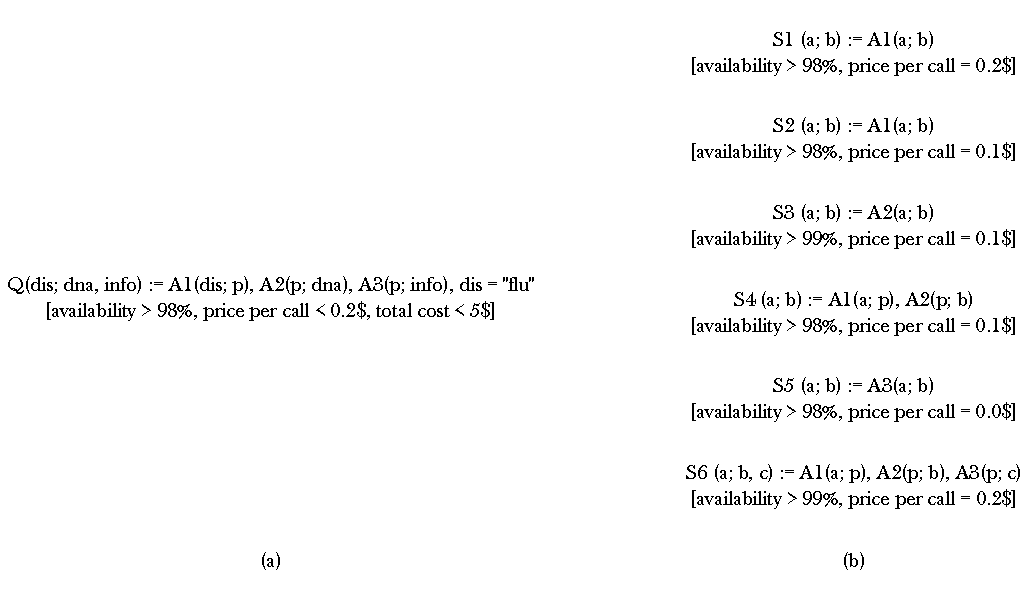
\includegraphics[scale=0.57]{query-and-services.pdf}
%\caption{\textit{Query} and \textit{concrete services} example.}\label{fig:queryandservices}
%\end{figure}
%
%Six \textit{concrete services} ($S1$, $S2$, $S3$, $S4$, $S5$ and $S6$) are are exemplified in the figure~\ref{fig:queryandservices} (right-site). $S1$ and $S2$ retrieve infected patients. $S3$ returns DNA information. $S4$ retrieves infected patients and DNA information given a disease name. $S5$ returns personal information. Finally, $S6$ retrieves patients' DNA and personal information given a disease name. Additionally, each \textit{concrete service} has its associated quality measures.

%The user provides a disease name and expects to retrieve the DNA and personal
%information of patients infected by the given disease. The query execution plan
%begins by retrieving infected patients ($GetPatients$). This operation returns patients' ids $p$. The abstract services $GetDNA$ and $GetInfo$ use patient ids to return their DNA and personal information ($dna$ and $info$).
%\textit{A user wants to retrieve patients DNA and personal information from patients infected by the disease ``flu'', using services with availability higher than 98\%, price per call less than 0.2\$ and total cost less than 2\$.}
%The query can be specified in terms of previous defined abstract services ($GetPatients$, $GetDNA$ and $GetInfo$) as follows. 
%The query $Q$ has an input parameter $d$ and an output parameter $dna$. 
%These \textit{head} variable are used in the \textit{abstract services} $diseasePatients$ and $DNAinformation$. 
%The local variable $p$ is an output in $diseasePatients$ and it is used as input in $GetDNA$.
%The query contains a constraint $d$ (disease name) equal to $flu$, and three user preferences $availability$ higher than 98 percent, $price \ per \ call$ less than 2 cents, and $total \ cost$ less than 2 dollars.


\subsection{Overview on the algorithm}
The main function of the \textit{Rhone} is described in the algorithm
\ref{algo-rhone}.
The input data for this function is a query, which includes a set of user preferences, and a set of concrete services. The result is a set of rewriting of the query in terms of concrete services, fulfilling the user preferences.

\begin{algorithm}
\small
\caption{ - RHONE}
\label{algo-rhone}
\begin{algorithmic}[1]
\REQUIRE A query $Q$, a set of user preferences, and a set of concrete services $\bigS$.
\ENSURE A set of rewritings $R$ that matches with the query and fulfill the user preferences.
\STATE \textbf{function} $\mathit{rhone} (Q, \bigS)$
 \STATE  $\bigLS \leftarrow \mathit{SelectCandidateServices}(Q, \bigS)$ \label{rhone:buildPCD}
 \STATE  $\bigLCSD \leftarrow CreateCSDs(Q, \bigLS)$
 \STATE  $I \leftarrow CombineCSDs(\bigLCSD)$
 \STATE $R\leftarrow ProduceRewritings(Q, I)$
    \STATE \textbf{return} $R$
\STATE \textbf{end function}
\end{algorithmic}
\end{algorithm}

In the first step, the algorithm looks for concrete services that 
can be matched with the query (line 2), resulting in a set of candidate concrete
services. For this set of services, the Rhone tries to create 
\textit{concrete services description} (CSD) for each service (line 3). 
A CSD is a structure that maps a concrete service to the query, or part of it. 
The  result of this step is a list of CSDs.
Given all produced CSDs  (line 4), they are combined among each other to
generate lists of CSD combinations, in each element represents a possible
rewriting.
Finally, given the list of combinations, the \textit{Rhone} identifies the
ones matching with the query and fulfilling the user preferences (line 5).
% The final step (lines 5) identifies which lists of CSDs are a valid rewriting of the user query given the list of lists of CSDs.
%A combination of CSDs is a valid rewriting if: (i) they cover all abstract services in the query; and 
%(ii) there is mapping to all head variables in the query (implemented by the function \textit{isRewriting}$(Q, p)$ %- line 8).
%The originality of our algorithm concerns the aggregation function (\agg{Q}).
%It is responsible to check and increment \textit{composed measures} (if present in the query). 
%This means for each element in the CSD list the value of \textit{composed measure} is incremented (line 10), and rewritings are produced while the values of these measures are respected (line 7). 
%The final result is a list of valid rewriting (line 5). 
In the next sections, each phase of the algorithm is described in detail. 

\subsection{Selecting services}

One contribution of our approach concerns the services selection process. Services are selected based on the user preferences and on the services' quality aspects collected from service level agreements.
While selecting services, the algorithm deals with three matching problems: \textit{measures} matching, \textit{abstract service} matching and \textit{concrete service} matching.
\bigskip

\noindent \textbf{Definition 3 (Measures matching)}.
Given a \textit{user preference} $P_{i}$ and a service's quality measure $Q_{j}$, a matching between them can be made if: (\textit{i}) the identifier $c_{i}$ in $P_{i}$ has the same name of $c_{j}$ in $Q_{j}$; and
(\textit{ii}) the evaluation of $Q_{j}$, denoted $eval(Q_{j})$, must satisfy the evaluation of $P_{i}$ ($eval(P_{i})$). In other words, $eval(Q_{j}) \subset eval(P_{i})$.
\bigskip

\noindent \textbf{Definition 4 (\textit{Abstract service} matching)}.
Given two abstract services $A_{i}$ and $A_{j}$, a match between \textit{abstract services} occurs when an \textit{abstract service} $A_{i}$ can be matched to $A_{j}$, denoted $A_{i} \equiv A_{j}$, according to the following conditions: 
(\textit{i}) $A_{i}$ and $A_{j}$ must have the same abstract function name; 
(\textit{ii}) the number of input variables of $A_{i}$, denoted $vars_{input}(A_{i})$, is equal or higher than the number of input variables of $A_{j}$ ($vars_{input}(A_{j})$); and 
(\textit{iii}) the number of output variables of $A_{i}$, denoted $vars_{output}(A_{i})$, is equal or higher than the number of output variables of $A_{j}$ ($vars_{output}(A_{j})$).
\bigskip

\noindent \textbf{Definition 5 (\textit{Concrete service} matching)}.
A \textit{concrete service} $S$ can be matched with the \textit{query} $Q$ according to the following conditions:
(\textit{i}) $\forall A_{i}  \ s. \ t. \lbrace\ A_{i} \in \ S\rbrace, \ \exists \ A_{j} \ $ $s. \ t. \lbrace\ A_{j} \in \ Q\rbrace, \ where \ A_{i} \equiv A_{j}.$ For all \textit{abstract services} $A_{i}$ in $S$, there is one \textit{abstract service} $A_{j}$ in $Q$ that satisfies the \textit{abstract service} matching problem (Definition 4); and (\textit{ii}) for all \textit{single preferences} $P_{i}$ in $Q$, there is one
\textit{service quality measure} $Q_{i}$ in $S$ that satisfies the \textit{measures} matching problem (Definition 3).


The process of selecting candidate concrete services
is described in the algorithm~\ref{selectingservices}.
Given the query $Q$ and a set of concrete services $\bigS$, the algorithm
looks for concrete services that can be used in the rewriting process.
Each selected service should satisfy the user preferences in $Q$ (line 4), and match with the query (line 7).
The services that satisfy all the matching problems are included in a set of candidate concrete services $\bigLS$ (line 12-13) which probably can be used in the rewriting process.

%The process of selecting candidate concrete services
%is described in the algorithm~\ref{selectingservices}.
%Given the query $Q$ and a set of concrete services $\bigS$, the algorithm
%looks for concrete services that can be used in the rewriting process.
%While iterating all concrete services in the list $\bigS$ (line 3), firstly,
%each service is checked to analyze if all its quality measures satisfies the user preferences
%in $Q$ (line 4). If it satisfies, each abstract service in $S_{i}$ is checked to confirm if 
%it matches or not with the query (lines 6-11). Once the service satisfies all the matching 
%problems, a set of candidate concrete services is produced (line 12-13). The result
%is a list of \textit{candidate concrete services} $\bigLS$ which
%probably can be used in the rewriting process (line 17).

\begin{algorithm}
%\small
\caption{ - Select candidate services}
\label{selectingservices}
\begin{algorithmic}[1]
\REQUIRE A query $Q$ and a set of concrete services $\bigS$.
\ENSURE A set of candidate concrete services $\bigLS$ that can be used in the rewriting process and fulfill the user preferences.
\STATE \textbf{function} $\mathit{SelectCandidateServices} (Q, \bigS)$
\STATE $\bigLS \leftarrow \emptyset$
\FORALL  {$S_{i}$ in $\bigS$}
	\IF {$\mathit{SatisfyQualityMeasures(Q, S_{i})}$}
		\STATE $b \leftarrow \mathit{true}$		
		\FORALL  {$A_{j}$ in $S_{i}$}
			\IF {$Q.\mathit{notContains(A_{i})}$}
				\STATE $b \leftarrow \mathit{false}$	
				\STATE $\mathit{break}$
			\ENDIF
		\ENDFOR
		\IF {$b = true$}
			\STATE $\bigLS \leftarrow \bigLS \cup \lbrace S_{i} \rbrace$	
		\ENDIF
	\ENDIF
\ENDFOR
\STATE \textbf{return} $\bigLS$
\STATE \textbf{end function}
\end{algorithmic}
\end{algorithm}

Let us consider the \textit{query} and \textit{concrete services} in our medical scenario (see figure~\ref{fig:queryandservices-selecting}).
The \textit{Rhone} iterates in the \textit{concrete service} list looking for services satisfying the matching problems.
Taking into account the \textit{query} and \textit{concrete services} specified in the \textit{Examples 1}, the \textit{concrete services} $S2$ and $S3$, $S4$ and $S5$ are selected as candidate concrete service once they satisfy all matching problems. However, $S1$, $S6$ and $S7$ are not select once their measures violate the user \textit{integration preference} `$price \ per \ call$'. In addition, $S7$ is not also selected because it contains a \textit{abstract service} that does not contribute to answer the \textit{query}.
\begin{figure}[h!]
\center
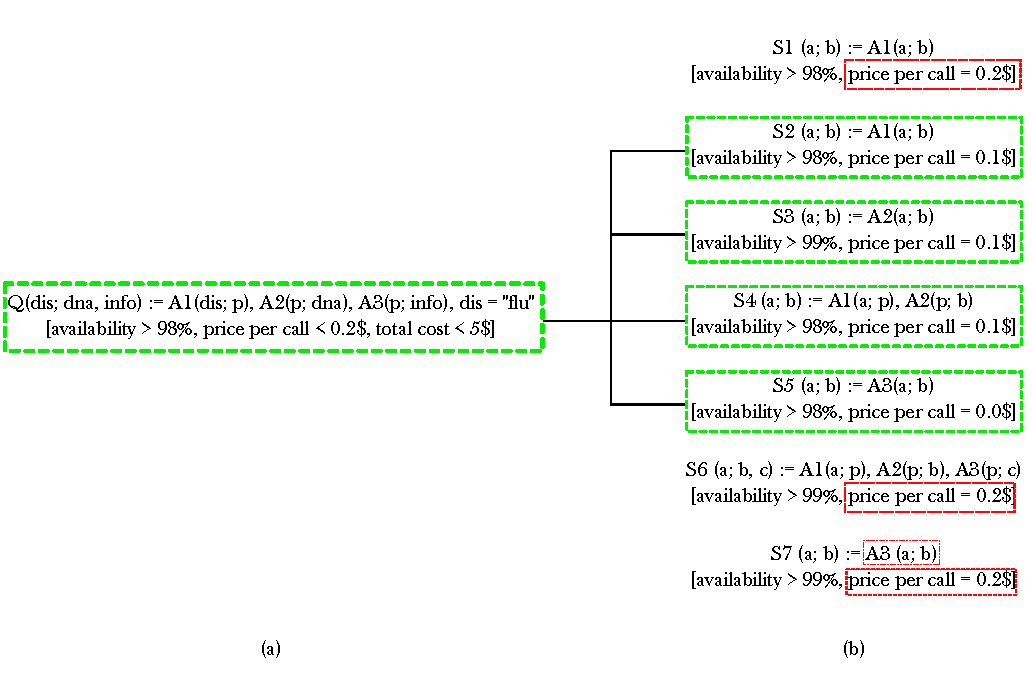
\includegraphics[scale=0.57]{query-and-services-selecting.pdf}
\caption{Service selection.}\label{fig:queryandservices-selecting}
\end{figure}

%
%\begin{example}
%The \textit{Rhone} iterates in the \textit{concrete service} list looking for services satisfying the matching problems.
%Taking into account the \textit{query} and \textit{concrete services} specified in the \textit{Examples 1}, the \textit{concrete services} $S2$ and $S3$, $S4$ and $S5$ are selected as candidate concrete service once they satisfy all matching problems. However, $S1$ and $S6$ are not select once it measures violate the user \textit{integration preference} $price per call$ as illustrated in the figure~\ref{fig:queryandservices-selecting}.
%\begin{figure}[h!]
%\center
%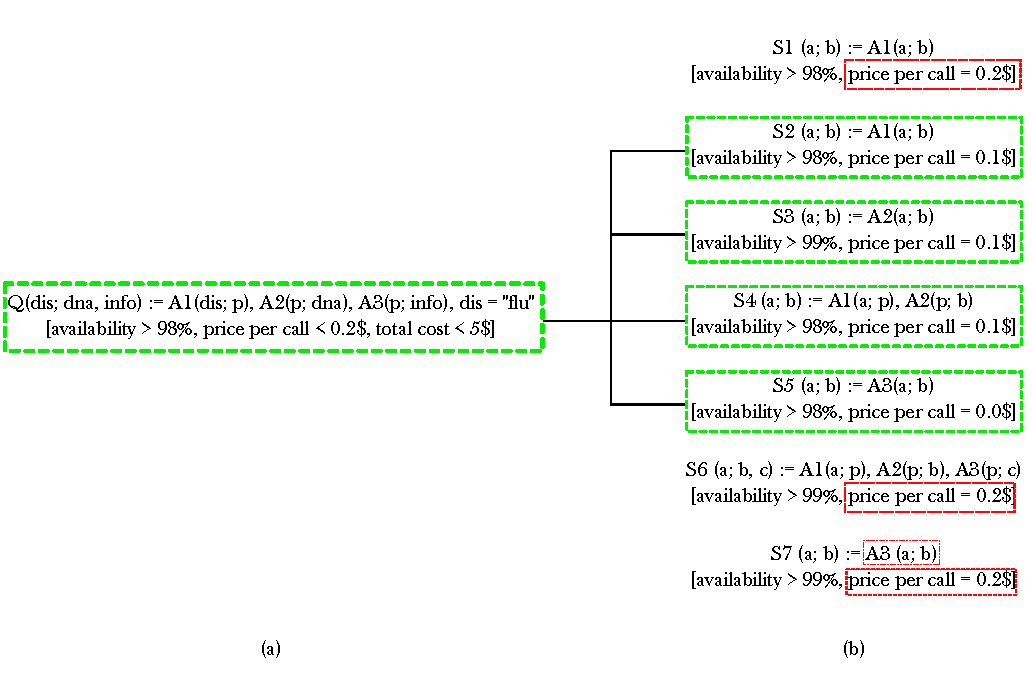
\includegraphics[scale=0.57]{query-and-services-selecting.pdf}
%\caption{Service selection.}\label{fig:queryandservices-selecting}
%\end{figure}
%\qed
%\end{example}

%\begin{algorithm}
%%\small
%\caption{ - Satisfy quality measures}
%\label{satisfymeasures}
%\begin{algorithmic}[1]
%\REQUIRE A query $Q$ and a concrete services $S_{i}$.
%\ENSURE A boolean value. \textit{True}, if the service satisfies the user preferences. \textit{False}, otherwise.
%\STATE \textbf{function} $\mathit{SatisfyQualityMeasures (Q, S_{i})}$
%\STATE to do
%%\STATE $\bigLS \leftarrow \emptyset$
%%\FORALL  {$S_{i}$ in $\bigS$}
%%	\IF {$\mathit{SatisfyQualityMeasures(Q, S_{i})}$}
%%		\STATE $b \leftarrow \mathit{true}$		
%%		\FORALL  {$A_{j}$ in $S_{i}$}
%%			\IF {$Q.\mathit{notContains(A_{i})}$}
%%				\STATE $b \leftarrow \mathit{false}$	
%%				\STATE $\mathit{break}$
%%			\ENDIF
%%		\ENDFOR
%%		\IF {$b = true$}
%%			\STATE $\bigLS \leftarrow \bigLS \cup \lbrace S_{i} \rbrace$	
%%		\ENDIF
%%	\ENDIF
%%\ENDFOR
%\STATE \textbf{return} $true$
%\STATE \textbf{end function}
%\end{algorithmic}
%\end{algorithm}

%\textcolor{red}{NaO ESTa FALTANDO ALGO??? CONTINUAR EXPLICANDO O EXEMPLO}

\subsection{Candidate service description}

After producing the set of candidate concrete services, the next step 
creates candidate service descriptions (CSDs). 
A CSD maps abstract services and variables of a concrete service into abstract 
services and variables of the query. 

\noindent \textbf{Definition 6 (candidate service description)}.
A CSD is represented by an n-tuple:
\begin{center}
$\langle S, h, \varphi, G, P\rangle$
\end{center}
where $S$ is a \textit{concrete service}. 
\textit{h} are mappings between variables in the \textit{head} of $S$ to variables in the \textit{body} of $S$. 
$\varphi$ are mapping between variables in the \textit{concrete service} to variables in the \textit{query}.
$G$ is a set of \textit{abstract services} covered by $S$. 
$P$ is a set \textit{quality measures} associated to the service $S$. 
 
A CSD is created according to 4 rules: (\textit{i}) for all head variables in a
concrete service, the mapping $h$ from the head to the body definition must
exist; (\textit{ii}) Head variables in concrete services can be mapped to head
or local variables in the query; (\textit{iii}) Local variables in concrete
services can be mapped to head variables in the query; and (\textit{iv}) Local
variables in concrete services can be mapped to local variables in the query if and only if the concrete service covers all abstract services in the query that depend on this variable. The relation ``depends''  means that this an output local variable is used as input in another abstract service.

The algorithm~\ref{creatingcsds} describes the creation of CSDs. Given the query $Q$ and a list of candidate concrete services $\bigLS$, a list of CSDs $\bigLCSD$ is produced. A  CSD is created only for candidate concrete services in which the mappings rules are being satisfied (line 4).
%The list of CSDs (line 17) is used to build rewritings of the query.
%
%The algorithm~\ref{creatingcsds} describes the creation of CSDs. Given the query $Q$ and a list of candidate concrete services $\bigLS$, a list of CSDs $\bigLCSD$ is produced. 
%The algorithm iterates on each service in $\bigLS$ (line 3), verifying if the mappings rules are being satisfied (line 4). For the ones which satisfies the mapping rules, a fresh copy of the abstract services in the concrete service is done in $G$(lines 7-9) and a copy of the service quality measures in done in $P$ (lines 10-12). Then,
%a CSD is created (line 13), and added to the final list of CSDs $\bigLCSD$ (line 14).
%The result of this phase is a list of CSDs that can be used to build rewriting of the query (line 17).

\begin{algorithm}[h!]
%\small
\caption{ - Create candidate service descriptions (CSDs)}
\label{creatingcsds}
\begin{algorithmic}[1]
\REQUIRE A query $Q$ and a set of candidate concrete services $\bigLS$.
\ENSURE A set of candidate service descriptions (CSDs) $\bigLCSD$ that contains mappings from candidate concrete service to the query.
\STATE \textbf{function} $\mathit{CreateCSDs} (Q, \bigLS)$
\STATE $\bigLCSD \leftarrow \emptyset$
\FORALL  {$S_{i}$ in $\bigLS$}
	\IF {There are mappings $\mathit{h}$ and $\varphi$ from $S_{i}$ to $Q$}	
		\STATE $G \leftarrow \emptyset$	
		\STATE $P \leftarrow \emptyset$		
		\FORALL  {$A_{j}$ in $S_{i}$}
			\STATE $G \leftarrow G \cup \lbrace A_{j} \rbrace$ 
		\ENDFOR
		\FORALL  {$M_{k}$ in $S_{i}$}
			\STATE $P \leftarrow P \cup \lbrace M_{k} \rbrace$ 
		\ENDFOR
		\STATE $CSD := \langle S_{i}, h, \varphi, G, P \rangle$	
		\STATE $\bigLCSD \leftarrow \bigLCSD \cup \lbrace CSD \rbrace$	
	\ENDIF
\ENDFOR
\STATE \textbf{return} $\bigLCSD$
\STATE \textbf{end function}
\end{algorithmic}
\end{algorithm}

Given the candidate concrete services selected in the figure~\ref{fig:queryandservices-selecting}. The algorithm builds CSDs to concrete services satisfying the mapping rules ($S2$, $S3$ and $S5$). For instance, $CSD_{1}$ is produced to $S2$ as follows: 
$\langle S2, \ h = \lbrace a \rightarrow a, \ b \rightarrow b \rbrace, \ \varphi = \lbrace a \rightarrow dis, \ b \rightarrow p \rbrace, \ G = \lbrace A1 \rbrace, \ P = \lbrace availability > 98\%, \ price \ per \ call = 0.1\$ \rbrace \rangle$. However, a CSD for $S4$ is not build because it violates the rule for local variables. It contains a local variable ($p$) mapped to a local variable in the query. Consequently, $S4$ must cover all abstract services in the query depending on this variable, but the abstract service $A3$ is not covered.

%\begin{example}%[producing candidate services descriptions]
%Given the candidate concrete services selected in the \textit{Example 3}. The algorithm builds CSDs to concrete services satisfying the mapping rules. $S1$, $S3$ and $S4$ satisfy all mapping rules. Consequently, CSDs for them are created. For instance, $CSD_{1}$ is produced to $S1$ as follows: 
%$\langle S1, \ h = \lbrace d \rightarrow d, \ p \rightarrow p \rbrace, \ \varphi = \lbrace d \rightarrow dis, \ p \rightarrow p \rbrace, \ G = \lbrace GetPatients \rbrace, \ P = \lbrace availability > 99\%, \ price \ per \ call = 0.1\$ \rbrace \rangle$. However, a CSD for $S5$ is not build because it violates the rule for local variables. It contains a local variable ($p$) mapped to a local variable in the query. Consequently, $S5$ must cover all abstract services in the query depending on this variable, but the abstract service $GetInfo$ is not covered.
%\qed
%\end{example}
 

\subsection{Combining and producing rewritings}
Given the list of CSDs $\bigLCSD$ produced, the \textit{Rhone} produces all possible combinations of its elements. 
Building combinations $I$ (Algorithm 1, line 4) deals with a NP hard complexity problem.
The effort to process combinations increases while the number of CSDs and abstract services in the query increases.

%\begin{center}
%\begin{minipage}[t]{6cm}
%  \vspace{0pt}  
%  \begin{algorithm}[H]
%    \caption{Producing rewritings}
%    \begin{algorithmic}[1]
%\REQUIRE Query $Q$ and a list of CSDs list $I$.
%\ENSURE A set of rewritings $R$ that matches with the query and fulfill the user preferences.
%\STATE \textbf{function} $\mathit{ProduceRewritings} (Q, I)$
%	\STATE $R\leftarrow \emptyset$
%	\STATE ~\!\tqI{\agg{Q}} 
%    \STATE $p \leftarrow I.next()$
%    \WHILE {$p\ \neq\ \emptyset$ \AND ~\!\tqT{\agg{Q}}} 
%		\IF {\textit{isRewriting}$(Q, p)$}
%			\STATE $R\leftarrow R\,\cup \mathit{Rewriting}(p)$
%			\STATE ~\!\tqS{\agg{Q}}
%		\ENDIF
%		\STATE $p \leftarrow I.\mathit{next}()$
%	\ENDWHILE
%    \STATE \textbf{return} $R$
%\STATE \textbf{end function}
%\end{algorithmic}
%  \end{algorithm}
%\end{minipage}%
%\begin{minipage}[t]{6cm}
%  \vspace{0pt}
%  \begin{algorithm}[H]
%    \caption{Algo 1}
%    \begin{algorithmic}[1]
%\REQUIRE A query $Q$ and a set of candidate services descriptions $p$.
%\ENSURE A boolean value. \textit{True}, if the set $p$ is a rewriting of the query. \textit{False}, otherwise.
%\STATE \textbf{function} $\mathit{isRewriting} (Q, p)$
%\STATE  $\mathbf{let} \ p = \lbrace CSD_{1}, CSD_{2}, ..., CSD_{k} \rbrace$
%\IF {(a) The number of elements in the union $CSD_{1}.G_{1} \ \cup \ CSD_{2}.G_{2}, ..., \ \cup \ CSD_{k}.G_{k}$
%is equal to the number of abstract services in $Q$\\
%	(b) The intersection $CSD_{1}.G_{1} \ \cap \ CSD_{2}.G_{2}, ..., \ \cap \ CSD_{k}.G_{k}$ is empty}	
%	\STATE \textbf{return} $true$		
%\ENDIF
%\STATE \textbf{return} $false$
%\STATE \textbf{end function}
%\end{algorithmic}
%  \end{algorithm}
%\end{minipage}
%\end{center}

\begin{algorithm}
%\small
\caption{ - Producing rewritings}
\label{rewriting}
\begin{algorithmic}[1]
\REQUIRE A query $Q$ and a list of lists of CSDs $I$.
\ENSURE A set of rewritings $R$ that matches with the query and fulfill the user preferences.
\STATE \textbf{function} $\mathit{ProduceRewritings} (Q, I)$
	\STATE $R\leftarrow \emptyset$
	\STATE ~\!\tqI{\agg{Q}} 
    \STATE $p \leftarrow I.next()$
    \WHILE {$p\ \neq\ \emptyset$ \AND ~\!\tqT{\agg{Q}}} 
		\IF {\textit{isRewriting}$(Q, p)$}
			\STATE $R\leftarrow R\,\cup \mathit{Rewriting}(p)$
			\STATE ~\!\tqS{\agg{Q}}
		\ENDIF
		\STATE $p \leftarrow I.\mathit{next}()$
	\ENDWHILE
    \STATE \textbf{return} $R$
\STATE \textbf{end function}
\end{algorithmic}
\end{algorithm}

%
The last step identifies rewritings matching with the query and fulfilling the user preferences (Algorithm~\ref{rewriting}). %The set of rewritings $R$ is initialized empty (line 2).
%
%A combination of CSDs is a valid rewriting if: (i) they cover all abstract services in the query; and (ii) there is mapping to all head variables in the query (implemented by the function \textit{isRewriting}$(Q, p)$ - line 8).
%
Another contribution in our algorithm concerns the aggregation functions $~\!\tqI{\agg{Q}}$, $~\!\tqT{\agg{Q}}$ and $~\!\tqS{\agg{Q}}$.
They are responsible to initialize (line 3), check conditions (line 5) and increment (line 8) composed preferences defined by the user.
This means for each element in the CSD list $p$ the value of a composed measure is computed and incremented. 
Rewritings are produced while the user preferences are respected. 

The \textit{Rhone} algorithm verifies if a given CSD list $p$ is a rewriting
of the original query (Algorithm 4, line 6).
The algorithm~\ref{isrewriting} describes this process in detail. 
Given the CSD list $p$ (line 2), the function return $true$ if (\textit{i}) the number of
abstract services resulting from the union of all CSDs in $p$ is equals to
the number of abstract services in the query; and (\textit{ii}) the intersection
of all abstract services in each CSD on $p$ is empty.
It means that is forbidden to have abstract services replicated among the set $p$.

%%
%The last step identifies rewritings matching with the query and fulfilling the user preferences (Algorithm~\ref{rewriting}). The set of rewritings $R$ is initialized empty (line 2).
%%
%%A combination of CSDs is a valid rewriting if: (i) they cover all abstract services in the query; and (ii) there is mapping to all head variables in the query (implemented by the function \textit{isRewriting}$(Q, p)$ - line 8).
%%
%Another contribution in our algorithm concerns the aggregation functions $~\!\tqI{\agg{Q}}$, $~\!\tqT{\agg{Q}}$ and $~\!\tqS{\agg{Q}}$.
%They are responsible to initialize (line 3), check conditions (line 5) and increment (line 8) composed preferences defined by the user.
%This means for each element in the CSD list $p$ the value of a composed measure is computed and incremented. 
%Rewritings are produced while the user preferences are respected. 
%
%The \textit{Rhone} algorithm verifies if a given CSD list $p$ is a rewriting
%of the original query (line 6).
%The algorithm~\ref{isrewriting} describes this process in detail. 
%Given the CSD list $p$ (line 2), the function return $true$ if it is a
%rewriting of the query.
%$p$ is a rewriting if it satisfies two conditions: (\textit{i}) the number of
%abstract services resulting from the union of all CSDs in $p$ must be equals to
%the number of abstract services in the query; and (\textit{ii}) the intersection
%of all abstract services in each CSD on $p$ must be empty.
%It means that is forbidden to have abstract services replicated among the set $p$.

\begin{algorithm}[h!]
%\small
\caption{ - Validating a combination of CSDs}
\label{isrewriting}
\begin{algorithmic}[1]
\REQUIRE A query $Q$ and a set of candidate services descriptions $p$.
\ENSURE A boolean value. \textit{True}, if the set $p$ is a rewriting of the query. \textit{False}, otherwise.
\STATE \textbf{function} $\mathit{isRewriting} (Q, p)$
\STATE  $\mathbf{let} \ p = \lbrace CSD_{1}, CSD_{2}, ..., CSD_{k} \rbrace$
\IF {(a) The number of elements in the union $CSD_{1}.G_{1} \ \cup \ CSD_{2}.G_{2}, ..., \ \cup \ CSD_{k}.G_{k}$
is equal to the number of abstract services in $Q$\\
	(b) The intersection $CSD_{1}.G_{1} \ \cap \ CSD_{2}.G_{2}, ..., \ \cap \ CSD_{k}.G_{k}$ is empty}	
	\STATE \textbf{return} $true$		
\ENDIF
\STATE \textbf{return} $false$
\STATE \textbf{end function}
\end{algorithmic}
\end{algorithm}

Let us consider $CSD_{2}$, $CSD_{3}$ and $CSD_{5}$ are CSDs that refer to the concrete services $S2$, $S3$ and $S5$, respectively. The \textit{Rhone} produces combinations taking into account the part of the query covered by the service as follows:
\begin{flushleft}
$p_{1} = \lbrace CSD_{2} \rbrace$ \\
$p_{2} = \lbrace CSD_{2}, CSD_{3} \rbrace$ \\
$p_{3} = \lbrace CSD_{2}, CSD_{3}, CSD_{5} \rbrace$
\end{flushleft}
Given the combinations, the \textit{Rhone} checks if each one of them is a valid
rewriting of the original query.
\begin{itemize}
\item $p_{1}$ and $p_{2}$ are not valid rewritings; their number of abstract services do not match with the number of abstract services in the query.
\item $p_{3}$ is a valid rewriting; the number of abstract services matches and there is no repeated abstract service. 
\end{itemize}

%\begin{example}%[producing combinations and identifying rewritings] 
%Let us consider the CSDs $CSD_{1}$, $CSD_{3}$ and $CSD_{5}$ produced in the \textit{Example 4} refers to the concrete services $S1$, $S3$ and $S4$, respectively. The \textit{Rhone} produces combinations as follows:
%\begin{flushleft}
%$p_{1} = \lbrace CSD_{1} \rbrace$ \\
%$p_{2} = \lbrace CSD_{1}, CSD_{3} \rbrace$ \\
%$p_{3} = \lbrace CSD_{1}, CSD_{3}, CSD_{4} \rbrace$
%\end{flushleft}
%Given the combinations, the \textit{Rhone} checks if each one of them is a valid
%rewriting of the original query.
%\begin{itemize}
%\item $p_{1}$ and $p_{2}$ are not valid rewritings; their number of abstract services do not match with the number of abstract services in the query.
%\item $p_{3}$ is a valid rewriting; the number of abstract services matches and there is no repeated abstract service. 
%\end{itemize}
%\qed
%\end{example}
	
%	
%%
%%The input for the \textit{Rhone} algorithm is: (1) a query, and (2) a list of
%%concrete services.
%\\ \\
%\noindent \textit{Abstract service} describes the small piece of function that can be performed by a cloud service. For instance, retrieve patients, DNA information and personal information. The \textit{abstract service} is defined as $A \ (\overline{I}; \ \overline{O})$ where: 
%\begin{itemize}
%\item $A$ is a name which identifies the \textit{abstract service}.
%\item $\overline{I}$ and $\overline{O}$ are a set of comma-separated input and output parameters, respectively.
%\end{itemize}
%The table~\ref{table:abstractservices} exemplifies \textit{abstract services} concerning our medical scenario described in the section~\ref{sec:scenario}.
%%
%%
%\begin{table}[]
%\centering
%\begin{tabular}{|l|p{8cm}|l|}
%\hline
%\multicolumn{1}{|c|}{\textbf{\textit{Abstract service} name}} & \multicolumn{1}{c|}{\textbf{Description}} \\ \hline
%$A1 \ (x; \ y)$ & Given a disease name $x$, $A1$ returns a list of infected patients' id $y$. \\ \hline
%$A2 \ (w; \ z)$ & Given a patient id $w$, $A2$ returns her DNA information $z$. \\ \hline
%$A3 \ (w; \ a)$ & Given a patient id $w$, $A3$ returns her personal information $a$.\\ \hline
%$A4 \ (x; \ r)$ & Given a disease name $x$, $A4$ returns the most affected region $r$. \\ \hline
%\end{tabular}
%\caption{List of \textit{abstract services}.}
%\label{table:abstractservices}
%\end{table}
%%
%
%\noindent \textit{Concrete service}
%
%
%\begin{definition}[query]
%A query $Q$ is defined as a set of \textit{abstract services}, a set of \textit{constraints}, and a set of \textit{user preferences} in accordance with the grammar:
%%
%\begin{center}
%\small
%\begin{math}
%Q (\overline{I}_{h}; \overline{O}_{h}) := A_{1}(\overline{I}_{1l};
%\overline{O}_{1l}), A_{2}(\overline{I}_{2l}; \overline{O}_{2l}), ..,  A_{n}(\overline{I}_{nl}; \overline{O}_{nl}),C_{1},C_{2}, .., C_{m}[P_{1},P_{2}, .., P_{k}]
%\end{math}
%\end{center}
%%
%The left-hand of the definition is called the \textit{head} of the query; and the right-hand is called the \textit{body}. 
%%
%$\overline{I}$ and $\overline{O}$ are a set of comma-separated \textit{input} and \textit{output} parameters, respectively.
%%
%Parameters can be of two types: \textit{head} variables and \textit{local} variables.
%\textit{Head} variables are parameters appearing in the head of the query. They
%also appear in the body of the query.
%\textit{Local} variables are parameters appearing only in the body of the query.
%%
%The sets of input and output parameters tagged with a subscript $h$ or $l$ refer to head or local parameters, respectively.
%%The sets $\overline{I}_{h}$ and $\overline{O}_{h}$ refer to \textit{head} input and output variables, 
%%and the sets $\overline{I}_{l}$ and $\overline{O}_{l}$ refer to \textit{local} input and output variables.
%%Intuitively, $\overline{I}$ is the union of $\overline{I}_{h}$ and all $\overline{I}_{l}$ such as
%Two rules are applied to those parameters: the union and the intersection. 
%For instance, the union of head and local input variables builds $\overline{I}$ such as  
%$\overline{I}$ =  $\overline{I}_{h} \cup \lbrace\overline{I}_{1l},..,\overline{I}_{nl}\rbrace$; 
%the intersection of head and local input variables is never empty such as $\lbrace\overline{I}_{h} \cap \overline{I}_{1l} \cap \overline{I}_{2l},.., \cap \overline{I}_{nl}\rbrace \ \neq \ \emptyset$. 
%%is not empty which means that: (1) there are \textit{head} variable that are used on the \textit{abstract services} in the body definition; and (2) there are \textit{local variables} that are shared among the \textit{abstract services}. 
%The same example can be used to output variables.
%%The same rule can be applied to output variables: $\overline{O}$ =  $\overline{O}_{h} \cup \lbrace\overline{O}_{1l},..,\overline{O}_{nl}\rbrace$, and the intersection among $\overline{O}_{h}$ and all $\overline{O}_{l}$ is not empty.
%% 
%
%%\textit{Abstract services} ($A_{1}, A_{2}, .., A_{n}$) describe a set of basic service operations.
%%
%$C_{1}, C_{2}, .., C_{m}$ are \textit{constraints} over the \textit{input} and/or \textit{output} parameters. These constraints are used while querying the databases. 
%The \textit{user preferences} (over the services) are specified in $P_{1}, P_{2}, .., P_{k}$.  
%%
%$C_{i}$ and $P_{j}$ are in the form $x \otimes c$, where $x$ is a identifier; $c$ is a constant; and
%$\otimes \in\lbrace \geq, \leq, =, \neq, <, >\rbrace$.
%%
%\qed
%\end{definition}
%
%User preferences can be of two types, single and composed. Single preferences
%are associated directly to each service involved in the composition. Composed
%preferences are linked to the entire composition. They are defined in terms of
%single preferences. For instance, the total response time is a composed
%preference obtained by adding the response time of each service involved in the composition.
%
%\begin{example}
%%
%Let us suppose a query specification based on the scenario (section \ref{sec:scenario}). The decorations $?$ and $!$ differentiate input and output parameters, respectively. 
%%
%\begin{center}
%\small
%$Q(dis?; dna!, info!) := GetPatients(dis?; p!), GetDNA(p?; dna!), GetInfo(p?; info!)$
%\\
%$d = ``flu'' [availability > 98\%, \ price \ per \ call < 0.2\$, \ total \ cost < 2\$]$
%\end{center}
%%
%The user provides a disease name and expects to retrieve the DNA and personal
%information of patients infected by the given disease. The query execution plan
%begins by retrieving infected patients ($GetPatients$). This operation returns patients' ids $p$. The abstract services $GetDNA$ and $GetInfo$ use patient ids to return their DNA and personal information ($dna$ and $info$).
%%\textit{A user wants to retrieve patients DNA and personal information from patients infected by the disease ``flu'', using services with availability higher than 98\%, price per call less than 0.2\$ and total cost less than 2\$.}
%%The query can be specified in terms of previous defined abstract services ($GetPatients$, $GetDNA$ and $GetInfo$) as follows. 
%%The query $Q$ has an input parameter $d$ and an output parameter $dna$. 
%%These \textit{head} variable are used in the \textit{abstract services} $diseasePatients$ and $DNAinformation$. 
%%The local variable $p$ is an output in $diseasePatients$ and it is used as input in $GetDNA$.
%The query contains a constraint $d$ (disease name) equal to $flu$, and three user preferences $availability$ higher than 98 percent, $price \ per \ call$ less than 2 cents, and $total \ cost$ less than 2 dollars.
%\qed
%\end{example}
%
%\begin{definition}[concrete services]
%A concrete service ($S$) is defined as a set of 
%\textit{abstract services}, and by its \textit{quality measures} according to the grammar:
%%
%\begin{center}
%\begin{math}
%S (\overline{I}_{h}; \overline{O}_{h}) := A_{1}(\overline{I}_{1l}; \overline{O}_{1l}), A_{2}(\overline{I}_{2l}; \overline{O}_{2l}), ..,  A_{f}(\overline{I}_{fl}; \overline{O}_{fl})[M_{1},M_{2}, ..,M_{g}]
%\end{math}
%\end{center}
%%
%%A \textit{concrete service} definition is similar to the \textit{query} definition, excepting the fact that a \textit{concrete service} does not have constraints over input and output variables.
%%
%A \textit{concrete service} definition is similar to the \textit{query} definition, excepting it does not have constraints. Parameters type and rules are applied in the same way.
%%
%%
%%The left-hand of the definition is the \textit{head}; and the right-hand is the \textit{body}. 
%%
%%$\overline{I}$ and $\overline{O}$ are a set of comma-separated \textit{input} and \textit{output} parameters, respectively.
%%
%%Parameters can be of two types: \textit{head} variables (appearing in the head and in the body definition) and \textit{local} variables (appearing only in the body definition).
%%\textit{Head} variables are parameters appearing in the head of the query; they also appear in the body of the query.
%%\textit{Local} variables are parameters appearing only in the body of the query.
%%
%%The sets of input and output parameters tagged with a subscript $h$ or $l$ refer to head or local parameters, respectively.
%%
%%The sets $\overline{I}_{h}$ and $\overline{O}_{h}$ refer to \textit{head} input and output variables, 
%%and the sets $\overline{I}_{l}$ and $\overline{O}_{l}$ refer to \textit{local} input and output variables.
%%Intuitively, $\overline{I}$ is the union of $\overline{I}_{h}$ and all $\overline{I}_{l}$ such as
%%Two rules are applied to those parameters: the union and the intersection. 
%%For instance, the union of head and local input variables builds $\overline{I}$ such as  
%%$\overline{I}$ =  $\overline{I}_{h} \cup \lbrace\overline{I}_{1l},..,\overline{I}_{nl}\rbrace$; 
%%the intersection of head and local input variables is never empty such as $\lbrace\overline{I}_{h} \cap \overline{I}_{1l} \cap \overline{I}_{2l},.., \cap \overline{I}_{nl}\rbrace \ \neq \ \emptyset$. 
%%is not empty which means that: (1) there are \textit{head} variable that are used on the \textit{abstract services} in the body definition; and (2) there are \textit{local variables} that are shared among the \textit{abstract services}. 
%%Intuitively, the same example can be used to output variables.
%%The same rule can be applied to output variables: $\overline{O}$ =  $\overline{O}_{h} \cup \lbrace\overline{O}_{1l},..,\overline{O}_{nl}\rbrace$, and the intersection among $\overline{O}_{h}$ and all $\overline{O}_{l}$ is not empty.
%%
%Concrete services are also defined in terms of \textit{abstract services} ($A_{1}, A_{2}, .., A_{n}$).
%%\textit{Abstract services} ($A_{1}, A_{2}, .., A_{n}$) describes a set of basic service capabilities.
%They contain a set of service's quality aspects (quality measures) $M_{1},M_{2}, .., M_{g}$. These measures are  associated to the concrete service itself and reflect the quality aspects guaranteed by the service. These aspects and penalties for its violation are agreed between the service and the provider in the service level agreement (SLA).
%%
%%
%$M_{i}$ is in the form $x \otimes c$, where $x$ is a special class of identifiers associated to the services; $c$ is a constant; and $\otimes \in\lbrace \geq, \leq, =, \neq, <, >\rbrace$.
%\qed
%\end{definition}
%
%%\textcolor{red}{REVER DEFINI��O QUE EST� IGUAL A ANTERIOR}
%
%In this algorithm, we are assuming this inputs come from a previous phase in our approach.
%This phase allows (i) to extract the service's quality measures from SLAs; and (ii) to generate the expected input data according to the grammar.
%
%\begin{example}
%%
%Assuming the query $Q$ specified in the \textit{Example 1}, five concrete services (that could be composed to answer it) are exemplified below. 
%\begin{flushleft}
%\small
%$S1(d?; p!) := GetPatients(d?; p!)[availability > 99\%, \ price \ per \ call = 0.1\$]$ 
%\\
%$S2(d?; p!) := GetPatients(d?; p!)[availability > 97\%, \ price \ per \ call = 0.2\$]$
%\\
%$S3(p?; dna!) := GetDNA(d?; dna!)[availability > 98\%, \ price \ per \ call = 0.1\$]$
%\\
%$S4(p?; info!) := GetInfo(d?; dna!)[availability > 98\%, \ price \ per \ call = 0.1\$]$
%\\
%$S5(d?; dna!) := GetPatients(d?; p!), GetDNA(p?; dna!)[availability > 98\%, \ price \ per \ call = 0.1\$]$
%\end{flushleft}
%$S1$, $S2$, $S3$, $S4$ and $S5$ are different concrete services defined in terms of abstract services or composition of abstract services (\textit{i.e.} $S5$). Each concrete service is tagged with its own quality measures. $S1$ and $S2$ retrieve infected patients, but they differ on the quality measures. $S3$ returns DNA information from a given patient. $S4$ retrieves personal information from patients. Finally, $S5$ covers two abstract services. It returns infected patients and their DNA information. 
%%Here, it is important to highlight that the \textit{quality measures} are extract from service level agreement in a previous phase of our approach that is not the focus in this paper.
%\qed
%\end{example}
%
%%\textcolor{red}{N�O EST� FALTANDO ALGO??? CONTINUAR EXPLICANDO}
%
%\subsection{Overview on the algorithm}
%The main function of the \textit{Rhone} is described in the algorithm
%\ref{algo-rhone}.
%The input data for this function is a query, which includes a set of user preferences, and a set of concrete services. The result is a set of rewriting of the query in terms of concrete services, fulfilling the user preferences.
%
%\begin{algorithm}
%\small
%\caption{ - RHONE}
%\label{algo-rhone}
%\begin{algorithmic}[1]
%\REQUIRE A query $Q$, a set of user preferences, and a set of concrete services $\bigS$.
%\ENSURE A set of rewritings $R$ that matches with the query and fulfill the user preferences.
%\STATE \textbf{function} $\mathit{rhone} (Q, \bigS)$
% \STATE  $\bigLS \leftarrow \mathit{SelectCandidateServices}(Q, \bigS)$ \label{rhone:buildPCD}
% \STATE  $\bigLCSD \leftarrow CreateCSDs(Q, \bigLS)$
% \STATE  $I \leftarrow CombineCSDs(\bigLCSD)$
% \STATE $R\leftarrow ProduceRewritings(Q, I)$
%% \STATE ~\!\tqI{\agg{Q}} 
%%    \STATE $p \leftarrow I.next()$
%%    \WHILE {$p\ \neq\ \emptyset$ \AND ~\!\tqI{\agg{Q}}} 
%%      \IF {\textit{isRewriting}$(Q, p)$}
%%  \STATE $R\leftarrow R\,\cup \mathit{Rewriting}(p)$
%%  \STATE ~\!\tqS{\agg{Q}}
%%   \ENDIF
%%      \STATE $p \leftarrow I.\mathit{Next}()$
%% \ENDWHILE
%    \STATE \textbf{return} $R$
%\STATE \textbf{end function}
%\end{algorithmic}
%\end{algorithm}
%
%In the first step, the algorithm looks for concrete services that 
%can be matched with the query (line 2), resulting in a set of candidate concrete
%services. For this set of services, the Rhone tries to create 
%\textit{concrete services description} (CSD) for each service (line 3). 
%A CSD is a structure that maps a concrete service to the query, or part of it. 
%The  result of this step is a list of CSDs.
%Given all produced CSDs  (line 4), they are combined among each other to
%generate lists of CSD combinations, in each element represents a possible
%rewriting.
%Finally, given the list of combinations, the \textit{Rhone} identifies the
%ones matching with the query and fulfilling the user preferences (line 5).
%% The final step (lines 5) identifies which lists of CSDs are a valid rewriting of the user query given the list of lists of CSDs.
%%A combination of CSDs is a valid rewriting if: (i) they cover all abstract services in the query; and 
%%(ii) there is mapping to all head variables in the query (implemented by the function \textit{isRewriting}$(Q, p)$ %- line 8).
%%The originality of our algorithm concerns the aggregation function (\agg{Q}).
%%It is responsible to check and increment \textit{composed measures} (if present in the query). 
%%This means for each element in the CSD list the value of \textit{composed measure} is incremented (line 10), and rewritings are produced while the values of these measures are respected (line 7). 
%%The final result is a list of valid rewriting (line 5). 
%In the next sections, each phase of the algorithm is described in detail. 
%
%\subsection{Selecting services}
%
%One contribution of our approach concerns the services selection process. Services are selected based on the user preferences and on the services' quality aspects collected from service level agreements.
%While selecting services, the algorithm deals with three matching problems: \textit{measures} matching, \textit{abstract service} matching and \textit{concrete service} matching.
%
%\begin{definition}[measures matching]
%Given a \textit{user preference} $P_{i}$ and a service's quality measure $Q_{j}$, a matching between them can be made if: (\textit{i}) the identifier $c_{i}$ in $P_{i}$ has the same name of $c_{j}$ in $Q_{j}$; and
%(\textit{ii}) the evaluation of $Q_{j}$, denoted $eval(Q_{j})$, must satisfy the evaluation of $P_{i}$ ($eval(P_{i})$). In other words, $eval(Q_{j}) \subset eval(P_{i})$.
%\qed
%\end{definition}
%
%\begin{definition}[abstract service matching]
%Given two abstract services $A_{i}$ and $A_{j}$, a match between \textit{abstract services} occurs when an \textit{abstract service} $A_{i}$ can be matched to $A_{j}$, denoted $A_{i} \equiv A_{j}$, according to the following conditions: 
%(\textit{i}) $A_{i}$ and $A_{j}$ must have the same abstract function name; 
%(\textit{ii}) the number of input variables of $A_{i}$, denoted $vars_{input}(A_{i})$, is equal or higher than the number of input variables of $A_{j}$ ($vars_{input}(A_{j})$); and 
%(\textit{iii}) the number of output variables of $A_{i}$, denoted $vars_{output}(A_{i})$, is equal or higher than the number of output variables of $A_{j}$ ($vars_{output}(A_{j})$).
%\qed
%\end{definition}
%
%\begin{definition}[concrete service matching]
%A \textit{concrete service} $S$ can be matched with the \textit{query} $Q$ according to the following conditions:
%(\textit{i}) $\forall A_{i}  \ s. \ t. \lbrace\ A_{i} \in \ S\rbrace, \ \exists \ A_{j} \ $ $s. \ t. \lbrace\ A_{j} \in \ Q\rbrace, \ where \ A_{i} \equiv A_{j}.$ For all \textit{abstract services} $A_{i}$ in $S$, there is one \textit{abstract service} $A_{j}$ in $Q$ that satisfies the \textit{abstract service} matching problem (Definition 4); and (\textit{ii}) for all \textit{single preferences} $P_{i}$ in $Q$, there is one
%\textit{service quality measure} $Q_{i}$ in $S$ that satisfies the \textit{measures} matching problem (Definition 3).
%\qed
%\end{definition}
%
%
%The process of selecting candidate concrete services
%is described in the algorithm~\ref{selectingservices}.
%Given the query and a set of concrete services, the algorithm
%looks for concrete services that can be used in the rewriting process.
%While iterating all concrete services in the list $\bigS$ (line 3), firstly,
%each service is checked to analyze if all its quality measures satisfies the user preferences
%in $Q$ (line 4). If it satisfies, each abstract service in $S_{i}$ is checked to confirm if 
%it matches or not with the query (lines 6-11). Once the service satisfies all the matching 
%problems, a set of candidate concrete services is produced (line 12-13). The result
%is a list of \textit{candidate concrete services} $\bigLS$ which
%probably can be used in the rewriting process (line 17).
%
%\begin{algorithm}
%%\small
%\caption{ - Select candidate services}
%\label{selectingservices}
%\begin{algorithmic}[1]
%\REQUIRE A query $Q$ and a set of concrete services $\bigS$.
%\ENSURE A set of candidate concrete services $\bigLS$ that can be used in the rewriting process and fulfill the user preferences.
%\STATE \textbf{function} $\mathit{SelectCandidateServices} (Q, \bigS)$
%\STATE $\bigLS \leftarrow \emptyset$
%\FORALL  {$S_{i}$ in $\bigS$}
%	\IF {$\mathit{SatisfyQualityMeasures(Q, S_{i})}$}
%		\STATE $b \leftarrow \mathit{true}$		
%		\FORALL  {$A_{j}$ in $S_{i}$}
%			\IF {$Q.\mathit{notContains(A_{i})}$}
%				\STATE $b \leftarrow \mathit{false}$	
%				\STATE $\mathit{break}$
%			\ENDIF
%		\ENDFOR
%		\IF {$b = true$}
%			\STATE $\bigLS \leftarrow \bigLS \cup \lbrace S_{i} \rbrace$	
%		\ENDIF
%	\ENDIF
%\ENDFOR
%\STATE \textbf{return} $\bigLS$
%\STATE \textbf{end function}
%\end{algorithmic}
%\end{algorithm}
%
%\begin{example}
%The \textit{Rhone} iterates in the concrete service list looking for services satisfying the matching problems.
%Taking into account the query and concrete services specified in the \textit{Examples 1} and \textit{2}:  
%$S1$, $S3$, $S4$ and $S5$ are selected as candidate concrete service once they satisfy all matching problems. However, $S2$ is not select once it measures violate the user preference $availability$ which is higher than 97\% and the user expects higher than 98\%.
%\qed
%\end{example}
%
%%\begin{algorithm}
%%%\small
%%\caption{ - Satisfy quality measures}
%%\label{satisfymeasures}
%%\begin{algorithmic}[1]
%%\REQUIRE A query $Q$ and a concrete services $S_{i}$.
%%\ENSURE A boolean value. \textit{True}, if the service satisfies the user preferences. \textit{False}, otherwise.
%%\STATE \textbf{function} $\mathit{SatisfyQualityMeasures (Q, S_{i})}$
%%\STATE to do
%%%\STATE $\bigLS \leftarrow \emptyset$
%%%\FORALL  {$S_{i}$ in $\bigS$}
%%%	\IF {$\mathit{SatisfyQualityMeasures(Q, S_{i})}$}
%%%		\STATE $b \leftarrow \mathit{true}$		
%%%		\FORALL  {$A_{j}$ in $S_{i}$}
%%%			\IF {$Q.\mathit{notContains(A_{i})}$}
%%%				\STATE $b \leftarrow \mathit{false}$	
%%%				\STATE $\mathit{break}$
%%%			\ENDIF
%%%		\ENDFOR
%%%		\IF {$b = true$}
%%%			\STATE $\bigLS \leftarrow \bigLS \cup \lbrace S_{i} \rbrace$	
%%%		\ENDIF
%%%	\ENDIF
%%%\ENDFOR
%%\STATE \textbf{return} $true$
%%\STATE \textbf{end function}
%%\end{algorithmic}
%%\end{algorithm}
%
%%\textcolor{red}{NaO ESTa FALTANDO ALGO??? CONTINUAR EXPLICANDO O EXEMPLO}
%
%\subsection{Candidate service description}
%
%After producing the set of candidate concrete services, the next step 
%creates candidate service descriptions (CSDs). 
%A CSD maps abstract services and variables of a concrete service into abstract 
%services and variables of the query. 
%
%\begin{definition}[candidate service description]
%A CSD is represented by an n-tuple:
%\begin{center}
%$\langle S, h, \varphi, G, P\rangle$
%\end{center}
%where $S$ is a \textit{concrete service}. 
%\textit{h} are mappings between variables in the \textit{head} of $S$ to variables in the \textit{body} of $S$. 
%$\varphi$ are mapping between variables in the \textit{concrete service} to variables in the \textit{query}.
%$G$ is a set of \textit{abstract services} covered by $S$. 
%$P$ is a set \textit{quality measures} associated to the service $S$. 
%\qed
%\end{definition} 
% 
%A CSD is created according to 4 rules: (\textit{i}) for all head variables in a
%concrete service, the mapping $h$ from the head to the body definition must
%exist; (\textit{ii}) Head variables in concrete services can be mapped to head
%or local variables in the query; (\textit{iii}) Local variables in concrete
%services can be mapped to head variables in the query; and (\textit{iv}) Local
%variables in concrete services can be mapped to local variables in the query if and only if the concrete service covers all abstract services in the query that depend on this variable. The relation ``depends''  means that this an output local variable is used as input in another abstract service.
%
%The algorithm~\ref{creatingcsds} describes the creation of CSDs. Given the query $Q$ and a list of candidate concrete services $\bigLS$, a list of CSDs $\bigLCSD$ is produced. 
%The algorithm iterates on each service in $\bigLS$ (line 3), verifying if the mappings rules are being satisfied (line 4). For the ones which satisfies the mapping rules, a fresh copy of the abstract services in the concrete service is done in $G$(lines 7-9) and a copy of the service quality measures in done in $P$ (lines 10-12). Then,
%a CSD is created (line 13), and added to the final list of CSDs $\bigLCSD$ (line 14).
%The result of this phase is a list of CSDs that can be used to build rewriting of the query (line 17).
%
%\begin{algorithm}[h!]
%%\small
%\caption{ - Create candidate service descriptions (CSDs)}
%\label{creatingcsds}
%\begin{algorithmic}[1]
%\REQUIRE A query $Q$ and a set of candidate concrete services $\bigLS$.
%\ENSURE A set of candidate service descriptions (CSDs) $\bigLCSD$ that contains mappings from candidate concrete service to the query.
%\STATE \textbf{function} $\mathit{CreateCSDs} (Q, \bigLS)$
%\STATE $\bigLCSD \leftarrow \emptyset$
%\FORALL  {$S_{i}$ in $\bigLS$}
%	\IF {There are mappings $\mathit{h}$ and $\varphi$ from $S_{i}$ to $Q$}	
%		\STATE $G \leftarrow \emptyset$	
%		\STATE $P \leftarrow \emptyset$		
%		\FORALL  {$A_{j}$ in $S_{i}$}
%			\STATE $G \leftarrow G \cup \lbrace A_{j} \rbrace$ 
%		\ENDFOR
%		\FORALL  {$M_{k}$ in $S_{i}$}
%			\STATE $P \leftarrow P \cup \lbrace M_{k} \rbrace$ 
%		\ENDFOR
%		\STATE $CSD := \langle S_{i}, h, \varphi, G, P \rangle$	
%		\STATE $\bigLCSD \leftarrow \bigLCSD \cup \lbrace CSD \rbrace$	
%	\ENDIF
%\ENDFOR
%\STATE \textbf{return} $\bigLCSD$
%\STATE \textbf{end function}
%\end{algorithmic}
%\end{algorithm}
%
%\begin{example}%[producing candidate services descriptions]
%Given the candidate concrete services selected in the \textit{Example 3}. The algorithm builds CSDs to concrete services satisfying the mapping rules. $S1$, $S3$ and $S4$ satisfy all mapping rules. Consequently, CSDs for them are created. For instance, $CSD_{1}$ is produced to $S1$ as follows: 
%$\langle S1, \ h = \lbrace d \rightarrow d, \ p \rightarrow p \rbrace, \ \varphi = \lbrace d \rightarrow dis, \ p \rightarrow p \rbrace, \ G = \lbrace GetPatients \rbrace, \ P = \lbrace availability > 99\%, \ price \ per \ call = 0.1\$ \rbrace \rangle$. However, a CSD for $S5$ is not build because it violates the rule for local variables. It contains a local variable ($p$) mapped to a local variable in the query. Consequently, $S5$ must cover all abstract services in the query depending on this variable, but the abstract service $GetInfo$ is not covered.
%\qed
%\end{example}
%
%%\textcolor{red}{N�O EST� FALTANDO ALGO??? CONTINUAR EXPLICANDO O EXEMPLO}
% 
%
%\subsection{Combining and producing rewritings}
%Given the list of CSDs $\bigLCSD$ produced, the \textit{Rhone} produces all possible combinations of its elements. 
%Building combinations $I$ (Algorithm 1, line 4) deals with a NP hard complexity problem.
%The effort to process combinations increases while the number of CSDs and abstract services in the query increases.
%
%\begin{algorithm}
%\small
%\caption{ - Producing rewritings}
%\label{rewriting}
%\begin{algorithmic}[1]
%\REQUIRE A query $Q$ and a list of lists of CSDs $I$.
%\ENSURE A set of rewritings $R$ that matches with the query and fulfill the user preferences.
%\STATE \textbf{function} $\mathit{ProduceRewritings} (Q, I)$
%	\STATE $R\leftarrow \emptyset$
%	\STATE ~\!\tqI{\agg{Q}} 
%    \STATE $p \leftarrow I.next()$
%    \WHILE {$p\ \neq\ \emptyset$ \AND ~\!\tqT{\agg{Q}}} 
%		\IF {\textit{isRewriting}$(Q, p)$}
%			\STATE $R\leftarrow R\,\cup \mathit{Rewriting}(p)$
%			\STATE ~\!\tqS{\agg{Q}}
%		\ENDIF
%		\STATE $p \leftarrow I.\mathit{next}()$
%	\ENDWHILE
%    \STATE \textbf{return} $R$
%\STATE \textbf{end function}
%\end{algorithmic}
%\end{algorithm}
%
%%
%The last step identifies rewritings matching with the query and fulfilling the user preferences (Algorithm~\ref{rewriting}). The set of rewritings $R$ is initialized empty (line 2).
%%
%%A combination of CSDs is a valid rewriting if: (i) they cover all abstract services in the query; and (ii) there is mapping to all head variables in the query (implemented by the function \textit{isRewriting}$(Q, p)$ - line 8).
%%
%Another contribution in our algorithm concerns the aggregation functions $~\!\tqI{\agg{Q}}$, $~\!\tqT{\agg{Q}}$ and $~\!\tqS{\agg{Q}}$.
%They are responsible to initialize (line 3), check conditions (line 5) and increment (line 8) composed preferences defined by the user.
%This means for each element in the CSD list $p$ the value of a composed measure is computed and incremented. 
%Rewritings are produced while the user preferences are respected. 
%
%The \textit{Rhone} algorithm verifies if a given CSD list $p$ is a rewriting
%of the original query (line 6).
%The algorithm~\ref{isrewriting} describes this process in detail. 
%Given the CSD list $p$ (line 2), the function return $true$ if it is a
%rewriting of the query.
%$p$ is a rewriting if it satisfies two conditions: (\textit{i}) the number of
%abstract services resulting from the union of all CSDs in $p$ must be equals to
%the number of abstract services in the query; and (\textit{ii}) the intersection
%of all abstract services in each CSD on $p$ must be empty.
%It means that is forbidden to have abstract services replicated among the set $p$.
%
%\begin{algorithm}[h!]
%%\small
%\caption{ - Validating a combination of CSDs}
%\label{isrewriting}
%\begin{algorithmic}[1]
%\REQUIRE A query $Q$ and a set of candidate services descriptions $p$.
%\ENSURE A boolean value. \textit{True}, if the set $p$ is a rewriting of the query. \textit{False}, otherwise.
%\STATE \textbf{function} $\mathit{isRewriting} (Q, p)$
%\STATE  $\mathbf{let} \ p = \lbrace CSD_{1}, CSD_{2}, ..., CSD_{k} \rbrace$
%\IF {(a) The number of elements in the union $CSD_{1}.G_{1} \ \cup \ CSD_{2}.G_{2}, ..., \ \cup \ CSD_{k}.G_{k}$
%is equal to the number of abstract services in $Q$\\
%	(b) The intersection $CSD_{1}.G_{1} \ \cap \ CSD_{2}.G_{2}, ..., \ \cap \ CSD_{k}.G_{k}$ is empty}	
%	\STATE \textbf{return} $true$		
%\ENDIF
%\STATE \textbf{return} $false$
%\STATE \textbf{end function}
%\end{algorithmic}
%\end{algorithm}
%
%\begin{example}%[producing combinations and identifying rewritings] 
%Let us consider the CSDs $CSD_{1}$, $CSD_{3}$ and $CSD_{5}$ produced in the \textit{Example 4} refers to the concrete services $S1$, $S3$ and $S4$, respectively. The \textit{Rhone} produces combinations as follows:
%\begin{flushleft}
%$p_{1} = \lbrace CSD_{1} \rbrace$ \\
%$p_{2} = \lbrace CSD_{1}, CSD_{3} \rbrace$ \\
%$p_{3} = \lbrace CSD_{1}, CSD_{3}, CSD_{4} \rbrace$
%\end{flushleft}
%Given the combinations, the \textit{Rhone} checks if each one of them is a valid
%rewriting of the original query.
%\begin{itemize}
%\item $p_{1}$ and $p_{2}$ are not valid rewritings; their number of abstract services do not match with the number of abstract services in the query.
%\item $p_{3}$ is a valid rewriting; the number of abstract services matches and there is no repeated abstract service. 
%\end{itemize}
%\qed
%\end{example}